\section{Introduction}\label{sec:introduction}
Causal structure learning from multivariate time series (MTS) is a fundamental problem with diverse applications in traffic modeling \citep{cheng2023causaltime}, biology \citep{sachs2005causal}, climate science \citep{runge2019detecting}, or healthcare \citep{shen2020challenges}. However, identifying causal relationships in MTS poses several challenges. First, real-world time series are often non-stationary, exhibiting multiple unknown regimes, each potentially governed by different causal relationships. Examples include changing dependencies across climate conditions \citep{karmouche2023regime}, financial markets \citep{huang2020causal}, and epileptic seizure stages \citep{wang2024ictal}. Second, many MTS display complex noises, e.g., non-Gaussian or even heteroscedastic noise, whose variance depends on both instantaneous and lagged causes. This occurs in fMRI data \citep{seiler2017multivariate}, EEG measurements \citep{huizenga1995equivalent}, or financial data \citep{hamilton1994autoregressive}.

Recent causal discovery methods capture linear and nonlinear interactions with instantaneous and lagged effects \citep{runge2018causal, pamfil2020dynotears, sun2021nts}.  More recently,  Gong et al. \citep{gong2022rhino} and Wang et al. \citep{wang2023neural} explored structural equation models for a single stationary regime governed by a one causal graph with historically dependent noise, where noise variance depends solely on time-lagged variables, neglecting heteroscedasticity. 
%Such assumptions are frequently violated in real-world settings, including neuroscience \citep{wang2024ictal}, climate science \citep{gunther2022conditional} and finance \citep{hamilton1994autoregressive}. 
Existing multi-regime methods include RPCMCI \citep{saggioro2020reconstructing}, which identifies only linear, time-lagged interactions and requires prior knowledge of regime numbers and transitions; and CD-NOD \citep{huang2020causal}, which handles causal discovery from non-stationary MTS, but is limited to homoscedastic noise, cannot infer individual causal graph for each regime, and is incapable of identifying recurring regimes. CASTOR \citep{rahmanicausal}, infers both regime indices and separate causal graphs per regime, accommodating instantaneous and lagged causal relationships, yet it is still restricted to normal noise. Consequently, the previous methods cannot jointly infer the number of regimes, their indices, their causal graphs, nor effectively manage either non-Gaussian 
 or heteroscedastic noises.\looseness=-1 
\begin{figure}[t]
    \centering
    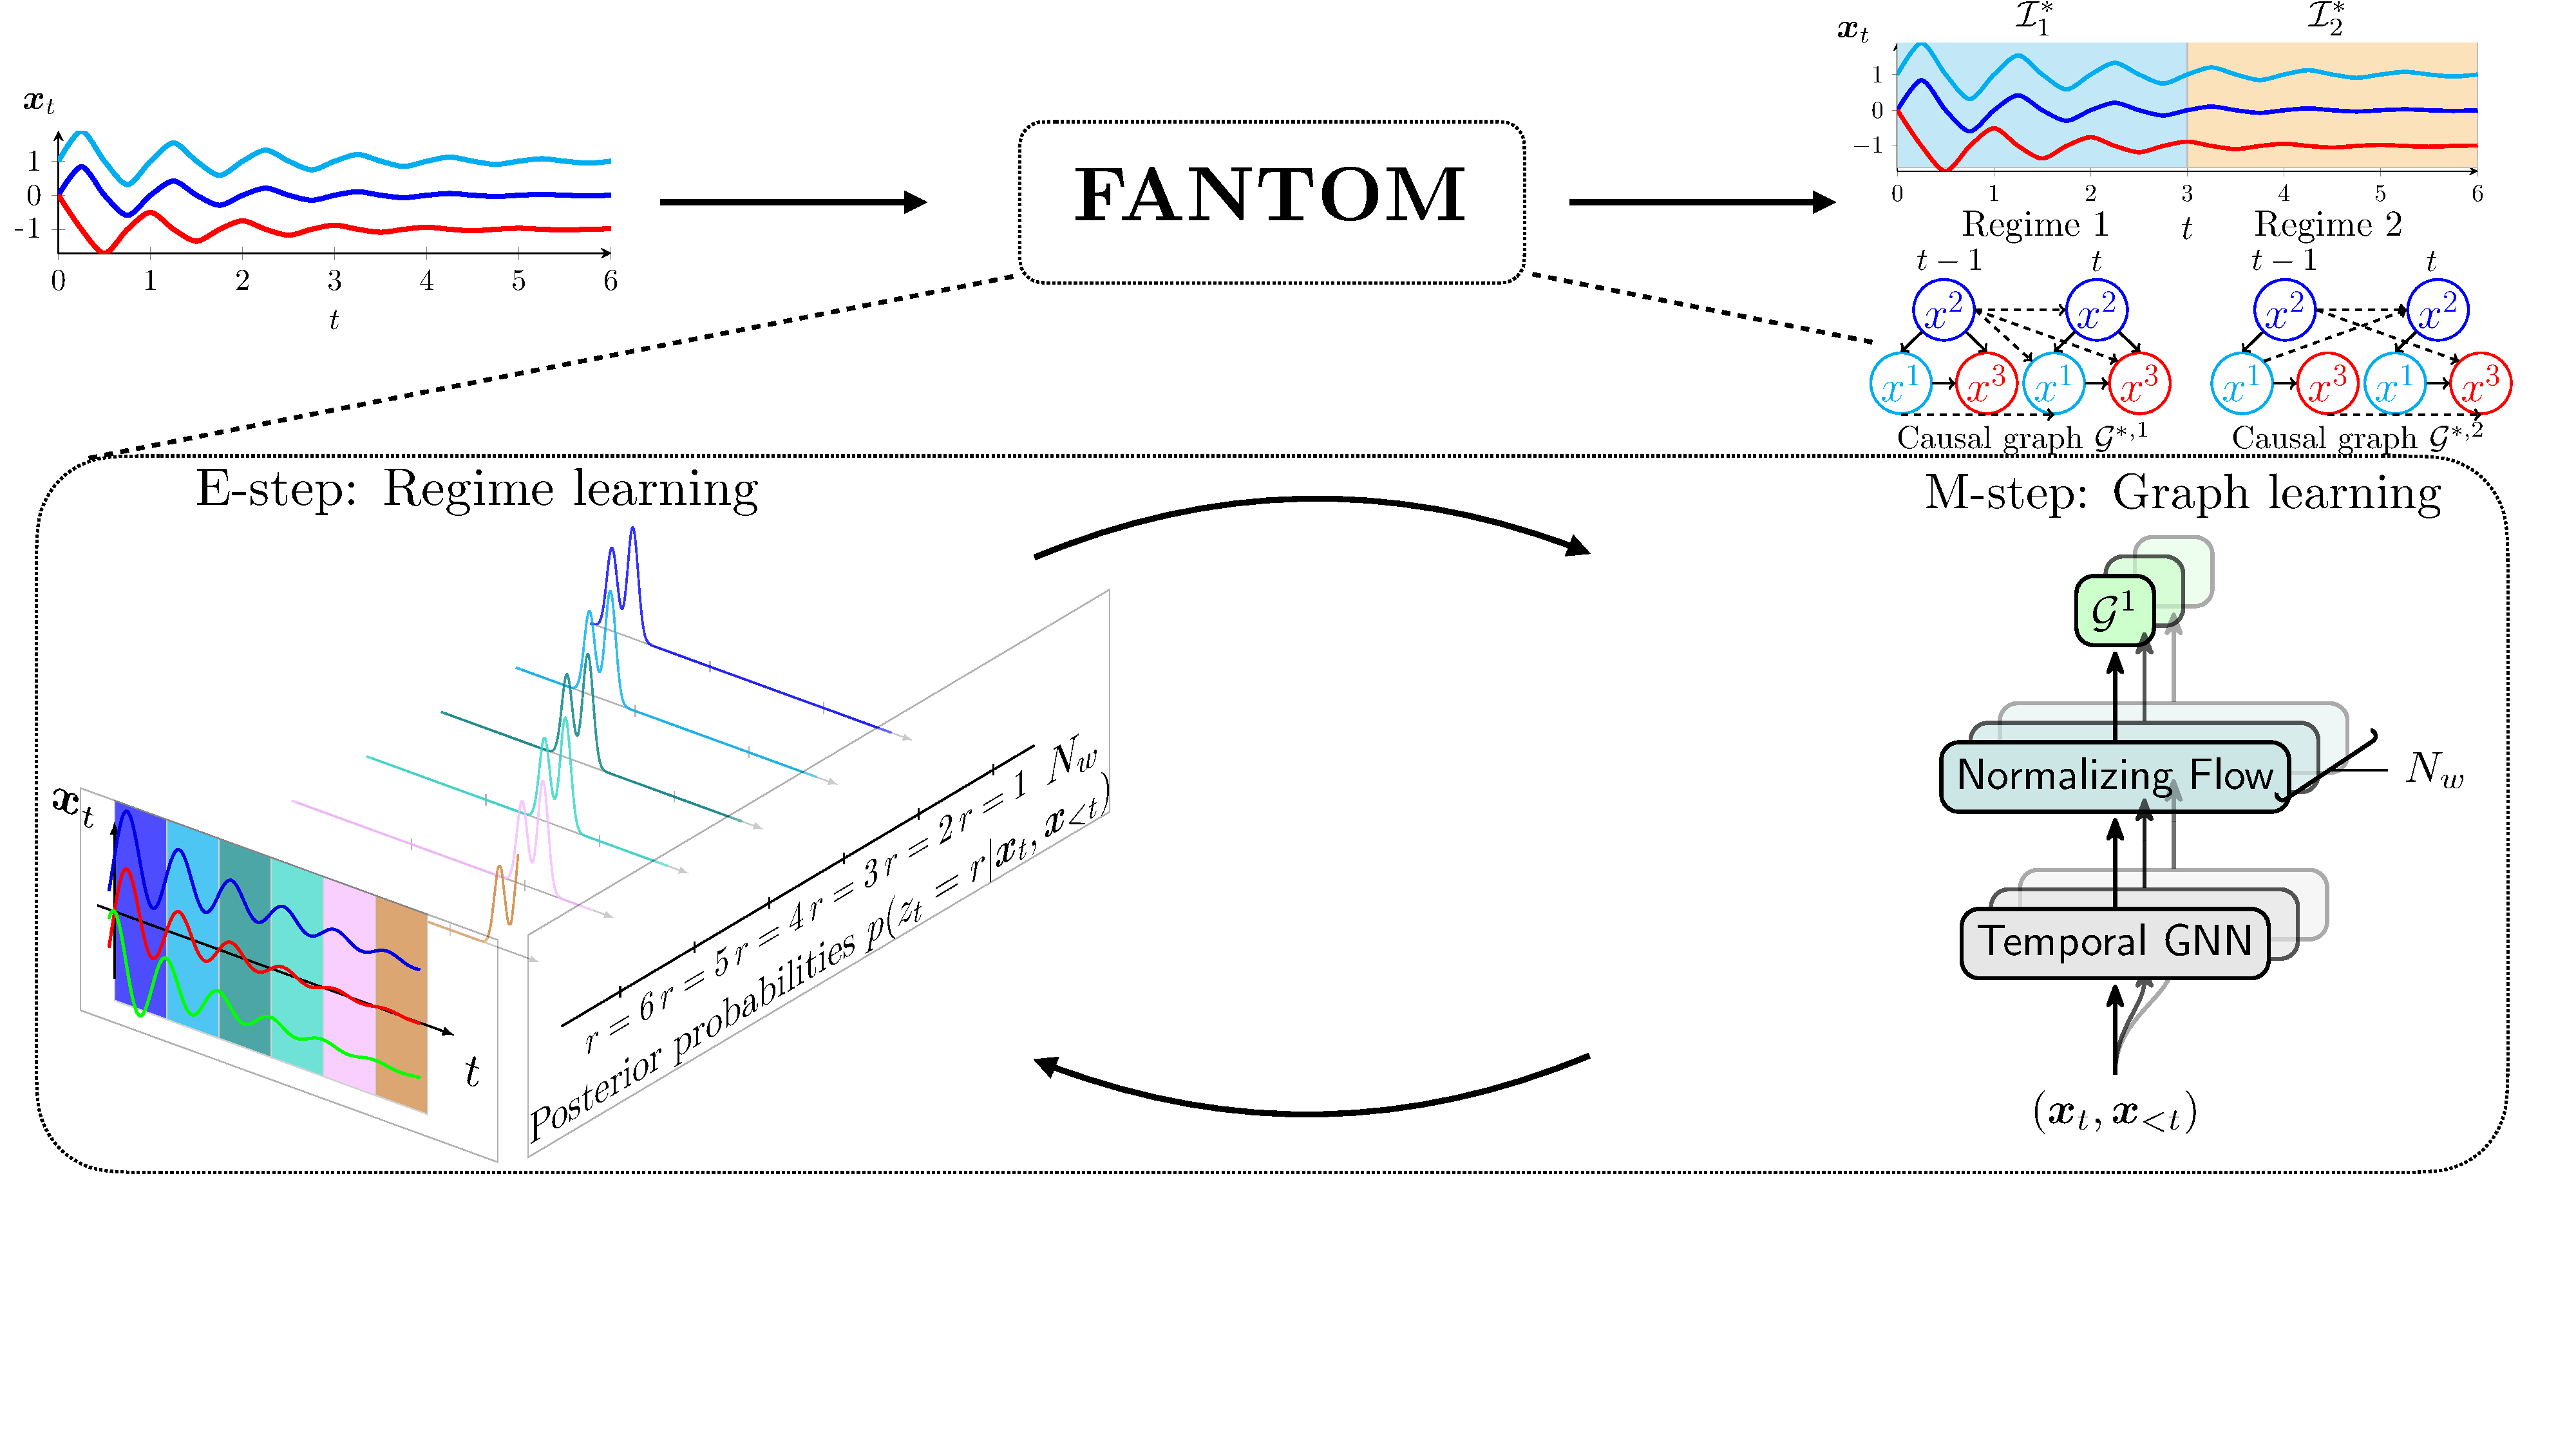
\includegraphics[width=1\linewidth]{figures/fantom_over_bigger_font.pdf}
    \caption{Illustration of FANTOM processing a MTS with two ground truth regimes (\(K=2\)). 
        The algorithm recovers the regime indices \(\mathcal{I}^{*}_1\) and \(\mathcal{I}^{*}_2\) and learns a temporal causal graph for each regime 
        (dashed edges represent time-lagged links; solid arrows indicate instantaneous links). 
        In the E-step, posterior probabilities \(p\bigl(z_t = r \mid \boldsymbol{x}_t, \boldsymbol{x}_{<t}\bigr)\) are estimated, 
        where \(z_t = r\) means \(\boldsymbol{x}_t\) belongs to regime \(r\). 
        The M-step then infers causal graphs within each regime. 
        Here, \(N_w\) is the number of regimes that converges to $K=2$.}
    \label{fig:fantom_over}
\end{figure}

To address these limitations, we propose FANTOM, a new framework for Structural Equation Models (SEMs) in multi-regime MTS under either non-Gaussian or heteroscedastic noises. FANTOM is, to the best of our knowledge, the first method to handle heteroscedasticity in both stationary and non-stationary MTS, as well as non-Gaussianity in non-stationary settings. Given a MTS with multiple regimes, FANTOM simultaneously learns each regime’s causal graph and mixing function, determines the number of regimes, and infers their indices (Figure~\ref{fig:fantom_over}). It uses a Bayesian Expectation Maximization (BEM) \citep{friedman2013bayesian} procedure to optimize the evidence lower bound (ELBO), alternatively assigning regime indices (Expectation step) and inferring causal relationships in each regime (Maximization step). Unlike Gaussian-based approaches, FANTOM employs conditional normalizing flows \citep{friedman2013bayesian}  to handle complex distributions and compute regime membership probabilities. It uses Bayesian structure learning that averages across all plausible graphs and naturally filters out spurious edges. Under mild assumptions, we prove that temporal heteroscedastic causal models are identifiable for both stationary and multi-regime MTS. Across extensive comparisons with existing multi-regime causal discovery methods, we show that FANTOM consistently achieves superior performance in structure learning and regime detection. Moreover, it outperforms stationary models, even when they are provided with ground-truth regime partitions, on synthetic and two real-world datasets. The main contributions of this paper can be summarized as follows:\looseness=-1 
\begin{itemize}
%\vspace{-3pt}
%\setlength\itemsep{-2pt}
\item We introduce FANTOM, a unified framework for causal discovery in multi-regime MTS that handles both homoscedastic non-Gaussian and heteroscedastic noises while simultaneously discovering the number of regimes, their indices, and their corresponding causal graphs.
\item Under mild assumptions in causal discovery, we prove identifiability of the temporal heteroscedastic causal models in the stationary case and show that the number of regimes, their indices, and their graphs are identifiable (up to permutation) in the non-stationary setting.
\item We demonstrate, via extensive experiments, that FANTOM outperforms state-of-the-art methods on both synthetic and real-world datasets.
\end{itemize}
\paragraph{Related work. }Many works tackle \textit{causal structure learning from stationary MTS}, Granger causality is the primary approach used for this purpose \citep{lowe2022amortized,bussmann2021neural}. However, it is unable to accommodate instantaneous effects. DYNOTEARS \citep{pamfil2020dynotears}, learns instantaneous and time lagged structures and leverages the acyclicity constraint, introduced by Zheng et al. in \citep{zheng2018dags}, to turn the DAG learning problem to a purely continuous optimization problem. However, DYNOTEARS is limited to linear SEMs. Runge et al. \citep{runge2020discovering} proposed a two-stage algorithm PCMCI+ that can scale to large time series, PCMCI+ is able also to handle non linear relationships. Neverthless, DYNOTEARS and PCMCI+ are restricted to homoscedastic noises where variance is a constant over time. For this reason, Rhino \citep{gong2022rhino} and SCOTCH \citep{wang2023neural} introduced models that tackle stationary MTS with historical noise, where the noise variance is a function of solely time lagged parents. However Rhino, DYNOTEARS and PCMCI+, cannot handle heteroscedastic noise and are limited to stationary MTS.

Several studies have sought to tackle the challenge of \textit{causal discovery in non-stationary MTS} \citep{huang2020causal, gunther2024causal, saggioro2020reconstructing, mameche2025spacetime}. Remarkably, Huang et al. \citep{huang2020causal} address the setting of time series composed of different regimes by modulating causal relationships through a regime index. CD-NOD detects change points and outputs a single summary causal graph, but it overlooks recurring regimes and provides neither regime-specific graphs nor their count. RPCMCI \citep{saggioro2020reconstructing} provides a graph for each regime, yet it assumes prior knowledge of the number of regimes, restricts edges to time-lagged links, and offers no identifiability guarantees. Balsells-Rodas et al. \citep{balsellsidentifiability} establish identifiability for first-order, regime-dependent causal discovery in multi-regime MTS with Gaussian noise and offer a practical algorithm, but their framework allows only a single time-lagged edge and excludes instantaneous links. Finally, CASTOR \citep{rahmanicausal} jointly infers regime labels and their causal graphs, capturing both instantaneous and lagged links, under an equivariant Gaussian noise assumption. However, none of these models can simultaneously learn the number of regimes, their indices, and their structures under non-Gaussian noise, nor do they offer identifiability guarantees. FANTOM fills this gap and even generalises to richer heteroscedastic noise settings while providing identifiability results. More detailed related work is provided in Appendix \ref{detaled_related}).